

\documentclass[final]{beamer}

\usepackage[
  orientation=landscape,
  size=custom,
  width=200,
  height=120,
  scale=2,
]{beamerposter}  %


\usetheme{confposter} %

\setbeamercolor{block title}{fg=ngreen,bg=white} %
\setbeamercolor{block body}{fg=black,bg=white} %
\setbeamercolor{block alerted title}{fg=white,bg=dblue!70} %
\setbeamercolor{block alerted body}{fg=black,bg=dblue!10} %


\newlength{\sepwid}
\newlength{\onecolwid}
\newlength{\threecolwid}
\setlength{\paperwidth}{200cm} %
\setlength{\paperheight}{120cm} %
\usepackage{etoolbox}
\makeatletter
\patchcmd{\beamer@@tmpl@headline}{wd=118cm}{wd=198cm}{}{}
\makeatother
\setlength{\sepwid}{0.001\paperwidth} %
\setlength{\onecolwid}{0.32\paperwidth} %
\setlength{\topmargin}{-0.5in} %

\usepackage{graphicx}  %
\graphicspath{{../../latex/images/}}

\usepackage{environ}
\usepackage{siunitx}

\usepackage{xcolor}
\definecolor{troyes}{rgb}{0.996078431372549, 0.9921568627450981, 0.9411764705882353}
\definecolor{frambo}{rgb}{0.7803921568627451, 0.17254901960784313, 0.2823529411764706}
\definecolor{lichen}{rgb}{0.5215686274509804, 0.7568627450980392, 0.49411764705882355}
\definecolor{canard}{rgb}{0.01568627450980392, 0.5450980392156862, 0.6039215686274509}
\definecolor{aurore}{rgb}{1.0, 0.796078431372549, 0.3764705882352941}
\definecolor{re}{rgb}{0.9607843137254902, 0.5725490196078431, 0.592156862745098}
\definecolor{gre}{rgb}{0.796078431372549, 0.8745098039215686, 0.5019607843137255}
\definecolor{blu}{rgb}{0.13725490196078433, 0.5803921568627451, 0.807843137254902}
\definecolor{ora}{rgb}{0.9803921568627451, 0.796078431372549, 0.5843137254901961}
\definecolor{yel}{rgb}{0.9490196078431372, 0.9411764705882353, 0.5450980392156862}

\newcommand{\colorbad}{frambo}
\newcommand{\colorgood}{canard}
\usetikzlibrary{automata, positioning, arrows, patterns}
\usepackage{pgfplots}
\newenvironment{figol}
{
\begin{tikzpicture}[thick]
    \begin{axis}[
    ]
        \draw[dashed] (1.85,-10)--(1.85,2);
        \draw[dashed] (-10,2)--(1.85,2);
        \draw (-0.5,-0.5) rectangle (0.5,0.5) node[pos=0.5] {$\mathcal{X}_t$};
        \draw [pattern=north west lines, pattern color=gray] (-10,-10) rectangle (-5,-5) node[pos=0.5] {$\mathcal{O}_1$};
        \draw [pattern=north west lines, pattern color=gray] (-5,-4) rectangle (1.85,-3) node[pos=0.5] {$\mathcal{O}_2$};
        \draw (-6,1) rectangle (-5,2) node[pos=0.5] {$\mathcal{A}$};
        \draw (-5,-3) rectangle (-4,-2) node[pos=0.5] {$\mathcal{B}$};
}
{
    \end{axis}
\end{tikzpicture}
}


\usepackage{booktabs} %

\usepackage{minted}

\usepackage{biblatex}
\addbibresource{biblio.bib}

\DeclareDatafieldSet{setall}{
  \member[datatype=literal]
  \member[datatype=name]
  \member[field=journal]%
}

\DeclareSourcemap{
  \maps[datatype=bibtex]{
    \map[overwrite, foreach={setall}]{
      \step[fieldsource=\regexp{$MAPLOOP},
            match=\regexp{\x{0131}\x{0300}},
            replace=\regexp{\x{00EC}}]
      \step[fieldsource=\regexp{$MAPLOOP},
            match=\regexp{\x{0131}\x{0301}},
            replace=\regexp{\x{00ED}}]
      \step[fieldsource=\regexp{$MAPLOOP},
            match=\regexp{\x{0131}\x{0302}},
            replace=\regexp{\x{00EE}}]
      \step[fieldsource=\regexp{$MAPLOOP},
            match=\regexp{\x{0131}\x{0308}},
            replace=\regexp{\x{00EF}}]
    }
  }
}

\AtEveryBibitem{%
    \clearfield{url}%
}

\usepackage[ruled,vlined]{algorithm2e}

\newcommand{\BnB}{Branch and bound}
\newcommand{\bnb}{branch and bound}

\newcommand{\Dsys}{\mathcal{S}}
\newcommand{\Hsys}{\mathcal{S}}
\newcommand{\hsyst}{discrete-time control hybrid system}
\newcommand{\Hsyst}{Discrete-time control hybrid system}
\newcommand{\states}{states}
\newcommand{\inputs}{inputs}
\DeclareMathOperator{\dom}{Dom} %
\newcommand{\lenub}{L}

\newcommand{\modename}{mode}
\newcommand{\modes}{\mathcal{Q}}
\newcommand{\target}{t}
\newcommand{\modeT}{q_t}
\newcommand{\statespace}{\mathcal{X}}
\newcommand{\dynto}{\rightsquigarrow}
\newcommand{\dyntop}{\rightsquigarrow'}
\newcommand{\dyntoh}{\widehat{\rightsquigarrow}}
\newcommand{\dyntot}{\widetilde{\rightsquigarrow}}
\newcommand{\dyntou}[1]{\stackrel[#1]{}{\rightsquigarrow}}
\newcommand{\dyntoup}[1]{\stackrel[#1]{}{\rightsquigarrow'}}
\newcommand{\dyntoupp}[1]{\stackrel[#1]{}{\rightsquigarrow}'}
\newcommand{\dyntouh}[1]{\stackrel[#1]{}{\widehat{\rightsquigarrow}}}
\newcommand{\dyntout}[1]{\stackrel[#1]{}{\widetilde{\rightsquigarrow}}}
\newcommand{\horizon}{H}
\newcommand{\deadline}{T}
\newcommand{\cost}{k}

\newcommand{\QcV}[1]{\mathcal{T}^Q_{c}{#1}}
\newcommand{\Qfun}{Q}
\newcommand{\Qfunv}{\hat{Q}}
\newcommand{\Qv}[3]{\Qfunv((#1, #2), #3)}
\newcommand{\Qvu}[5][\Qfun]{{#1}((#2, #3), (#4, #5))}
\newcommand{\policy}{\mu}

\DeclareMathOperator{\Dom}{Dom}
\newcommand{\valuefun}{J}

\usepackage{stackrel}

\DeclareMathOperator*{\Post}{Post}
\newcommand{\post}[2]{\Post_{\dyntou{#1}}(#2)}
\newcommand{\posth}[2]{\Post_{\dyntouh{#1}}(#2)}
\newcommand{\postt}[2]{\Post_{\dyntout{#1}}(#2)}
\newcommand{\posttwo}[2]{\Post_{\stackrel[#1]{2}{\rightsquigarrow}}(#2)}
\newcommand{\postone}[2]{\Post_{\stackrel[#1]{1}{\rightsquigarrow}}(#2)}

\usepackage{ifthen}
\newcommand{\emptytuple}{\emptyset}
\newcommand{\myemptyset}{\varnothing}
\newcommand{\tuplecat}[2]{(#1; #2)}
\newcommand{\tuple}[3]{\ifthenelse{\equal{#2}{1}}{\mathbf{#1}_{#3}}{({#1}_i)_{i=#2}^{#3}}}
\newcommand{\tuplep}[3]{\ifthenelse{\equal{#2}{1}}{\mathbf{#1}'_{#3}}{({#1}'_i)_{i=#2}^{#3}}}
\newcommand{\tuples}[3]{\ifthenelse{\equal{#2}{1}}{\mathbf{#1}^\star_{#3}}{({#1}^\star_i)_{i=#2}^{#3}}}

\usepackage{hyperref}



\title{Abstraction-based branch and bound approach to Q-learning for hybrid optimal control} %

\author{Beno\^it Legat$^*$, Jean Bouchat$^*$, Rapha\"el M. Jungers$^*$}

\institute{Summarising video available at \url{https://youtu.be/2bc0iHZFf24} \hspace{10em} $^*$ UCLouvain} %


\makeatletter
\let\@@magyar@captionfix\relax
\makeatother

\begin{document}

\addtobeamertemplate{block end}{}{\vspace*{2ex}} %
\addtobeamertemplate{block alerted end}{}{\vspace*{2ex}} %

\setlength\belowdisplayshortskip{2ex} %

\begin{frame}[t,fragile] %

\begin{columns}[t] %


\begin{column}{0.95\onecolwid} %
  \alert{Optimal control} problem for \alert{hybrid} system with \alert{affine} subsystems.
  State-space: $\mathcal{Q} \times \mathcal{X}$ for
  $\mathcal{X} \subseteq \mathcal{R}^{n_x}$
  and finite set $\mathcal{Q}$.
  \begin{block}{\BnB{} algorithm}
  \begin{algorithm}[H]
      \DontPrintSemicolon
      $\bar{\beta} \gets \infty$\tcp*{No upper bound (UB)}

      $\mathcal{N} \gets \{\emptytuple{}\}$\tcp*{Empty trajectory in priority queue}
      \While{$\mathcal{N} \neq \myemptyset$}{
        $\tuple{v}{1}{l} \gets h(\mathcal{N})$\tcp*{Heuristic picks trajectory}

          $\mathcal{N} \gets \mathcal{N} \setminus \{\tuple{v}{1}{l}\}$\tcp*{Remove from prority queue}

          \If{$\Qv{q_0}{x_0}{\tuple{v}{1}{l}} \le \bar{\beta}$\tcp*{branch LB $\le$ global UB}}{
              \For{$v' \in \mathcal{V}$}{
                  $\tuple{\hat{v}}{1}{\hat{l}}, \tuple{\hat{u}}{1}{\hat{l}}, \hat{\beta} \gets \beta(q_0, x_0, \tuplecat{\tuple{v}{1}{l}}{v'})$\tcp*{Any feasible solutions ?}
                  Q-learning for lower bound $Q$ along trajectory $\tuple{\hat{v}}{1}{\hat{l}}, \tuple{\hat{u}}{1}{\hat{l}}$\;

                  \If{$\hat{\beta} < \bar{\beta}$}{$\tuple{\bar{v}}{1}{\bar{l}}, \tuple{\bar{u}}{1}{\bar{l}}, \bar{\beta} \gets \tuple{\hat{v}}{1}{\hat{l}}, \tuple{\hat{u}}{1}{\hat{l}}, \hat{\beta}$\tcp*{Update UB}}


                  $\mathcal{N} \gets \mathcal{N} \cup \{\tuplecat{\tuple{v}{1}{l}}{v'}\}$\tcp*{Add to priority queue}
              }
          }
      }
      \Return{$\tuple{\bar{v}}{1}{\bar{l}}, \tuple{\bar{u}}{1}{\bar{l}}$}\;
  \end{algorithm}
  \end{block}


  \begin{block}{Exploration-exploitation trade-off}
    Upper bound $\beta$ obtained using \alert{MPC} with \alert{Lyapunov} function $L(q, x)$.
    Lyapunov function $L(q, x)$ is zero at the target, finite in some controlled invariant set around the target,
    infinite otherwise.

    The \alert{largest} the controlled invariant set, the \alert{faster} the algorithm gets upper bounds.

    Which \alert{heuristic} $h$ should be used ?
    \begin{description}
      \item[Exploration]:
        Priority to lowest lower bound.
        This needs a Lyapunov function with large controlled invariant set to still get upper bounds early ;
      \item[Exploitation]:
        Depth first search, break ties with lower bound.
        Quickly get upper bounds, even with poor Lyapunov function.
    \end{description}
  \end{block}

\end{column}


\begin{column}{0.96\onecolwid} %
  \begin{block}{Q-learning}
    Optimal control of \alert{hybrid} systems so
    Q-function is \alert{nonconvex}.
  \begin{center}
    \begin{tikzpicture}[scale=2, thick]
        \draw[->] (-11,0) -- (3,0) node[right] {$x$};
        \draw[->] (-10.5,-0.5) -- (-10.5,7);
        \draw[domain=-10:-5,smooth,variable=\x,blue] plot ({\x},{0.3*(\x*\x)+4.1*\x+17});
        \draw[domain=-5:2,smooth,variable=\x,blue] plot ({\x},{0.3*(\x*\x)+1.1*\x+2}) node[right] {$Q^\star(q,x)$};
        \draw[domain=-10:-4.57,densely dotted,variable=\x,red] plot ({\x},{0});
        \draw[domain=-4.57:0,variable=\x,red] plot ({\x},{0});
        \draw[domain=0:2,densely dotted,variable=\x,red] plot ({\x},{0});
        \draw[domain=-10:-4.57,variable=\x,red] plot ({\x},{-0.7*(\x+8)+3.4-1});
        \draw[domain=-4.57:-1,densely dotted,variable=\x,red] plot ({\x},{-0.7*(\x+8)+3.4-1});
        \draw[domain=-3:0,densely dotted,variable=\x,red] plot ({\x},{0.9*(\x+8)-7.2});
        \draw[domain=0:3,variable=\x,red] plot ({\x},{0.9*(\x+8)-7.2}) node[right] {$\tilde{Q}(q,x)$};
    \end{tikzpicture}
  \end{center}
    \alert{Gap} between polyhedral lower bound can be reduced by
    increasing \alert{horizon}~\cite{menta2020learning},
    or \alert{refining} the hybrid state-space abstraction:
  \begin{center}
    \begin{tikzpicture}[scale=2,thick]
        \draw[->] (-13.5,0) -- (3.5,0) node[right] {$x$};
        \draw[->] (-13,-0.5) -- (-13,7);
        \draw[domain=-10:-5,smooth,variable=\x,blue] plot ({\x},{0.3*(\x*\x)+4.1*\x+17});
        \node [blue] at (-10.75,6.5) {$Q^\star(q_a,x)$};
        \draw[domain=-5:2,smooth,variable=\x,blue] plot ({\x},{0.3*(\x*\x)+1.1*\x+2}) node[right] {$Q^\star(q_b,x)$};
        \draw[domain=-0.5:7,dashed,variable=\y] plot ({-5},{\y});
        \draw[domain=-10:-7.5,variable=\x,red] plot ({\x},{-0.7*(\x+8)+3.4-1});
        \draw[domain=-7.5:-4.6,densely dotted,variable=\x,red] plot ({\x},{-0.7*(\x+8)+3.4-1});
        \draw[domain=-10:-7.5,densely dotted,variable=\x,red] plot ({\x},{0.7*(\x+2)+5.9});
        \draw[domain=-7.5:-5,variable=\x,red] plot ({\x},{0.7*(\x+2)+5.9});
        \node [red] at (-11,3) {$\tilde{Q}(q_a,x)$};
        \draw[domain=-5:-1.344,variable=\x,red] plot ({\x},{-0.8*(\x+8)+5.325});
        \draw[domain=-1.344:0,densely dotted,variable=\x,red] plot ({\x},{-0.8*(\x+8)+5.325});
        \draw[domain=-4.6:-1.344,densely dotted,variable=\x,red] plot ({\x},{0});
        \draw[domain=-1.344:0,variable=\x,red] plot ({\x},{0});
        \draw[domain=-2:0,densely dotted,variable=\x,red] plot ({\x},{0.9*(\x+8)-7.2});
        \draw[domain=0:2,variable=\x,red] plot ({\x},{0.9*(\x+8)-7.2}) node[right] {$\tilde{Q}(q_b,x)$};
        \fill[pattern=north east lines, pattern color=gray] plot coordinates {(-7.4,2.05) (-4.55,0.1) (-1.6,0.1) (-5.05,2.8) (-5.05,3.65) (-7.4,2.05)};
    \end{tikzpicture}
  \end{center}
    \alert{Dual} obtained by solving a \alert{strong} formulation.
    Epigraph of the nonconvex \textcolor{blue}{$\tilde{Q}(q, x)$} below replaced
    by its convex hull: the epigraph of \textcolor{red}{$\Theta(x)$} below:
  \begin{center}
    \begin{tikzpicture}[scale=10,thick]
        \draw[->] (-0.25,0) -- (3.5,0) node[right] {$x$};
        \draw[->] (0,-0.25) -- (0,2.25);
        \draw[domain=0:1,variable=\x,blue] plot ({\x},{1});
        \draw[domain=0.5:1,variable=\y,blue] plot ({1},{\y});
        \draw[domain=1:2,variable=\x,blue] plot ({\x},{0.5});
        \draw[domain=0.5:2,variable=\y,blue] plot ({2},{\y});
        \draw[domain=2:3,variable=\x,blue] plot ({\x},{2}); %
        \draw[domain=0:1,variable=\x,,red] plot ({\x},{-0.5*\x+0.965});
        \draw[domain=1:2,variable=\x,,red] plot ({\x},{0.465});
        \draw[domain=2:3,variable=\x,,red] plot ({\x},{1.5*\x-2.535}) node at (3.1,1.5) {$\Theta(x)$};
        \node[blue,above] at (0.5,1) {$\tilde{Q}(q_1, x)$};
        \node[blue,above] at (1.5,0.5) {$\tilde{Q}(q_2, x)$};
        \node[blue,above] at (2.5,2) {$\tilde{Q}(q_3, x)$};
        \node at (0.5,-0.25) {$\dom(1)$};
        \draw[<->|] (0,-0.075) -- (1,-0.075);
        \node at (1.5,-0.25) {$\dom(2)$};
        \draw[<->|] (1,-0.075) -- (2,-0.075);
        \node at (2.5,-0.25) {$\dom(3)$};
        \draw[<->|] (2,-0.075) -- (3,-0.075);
    \end{tikzpicture}
  \end{center}
  \end{block}

\end{column}

\begin{column}{\sepwid}\end{column} %

\begin{column}{1.05\onecolwid} %

  \begin{block}{Numerical results}
  Number of iterations of \BnB{} algorithm:
  \begin{center}
    \begin{tabular}{c|c|c}
        Bellman-like Q-function & \# iterations for $\mathcal{I}_1$ & \# iterations for $\mathcal{I}_2$\\
        \hline
        $Q_1$ & \num{197234} & \num{9388410}\\
        $Q_2$ & \num{1076} & \num{96}\\
        $Q_2$ with learning & \num{789} & \num{75}\\
        $Q_2$ learning on $\mathcal{I}_1$ & \num{782} & \num{74}\\
        $Q_2$ learning on $\mathcal{I}_2$ & \num{800} & \num{74}\\
    \end{tabular}
  \end{center}

  Feasible solutions for $\mathcal{I}_1$ (left) and $\mathcal{I}_2$ (right) with increasingly better bounds:
  \begin{center}
    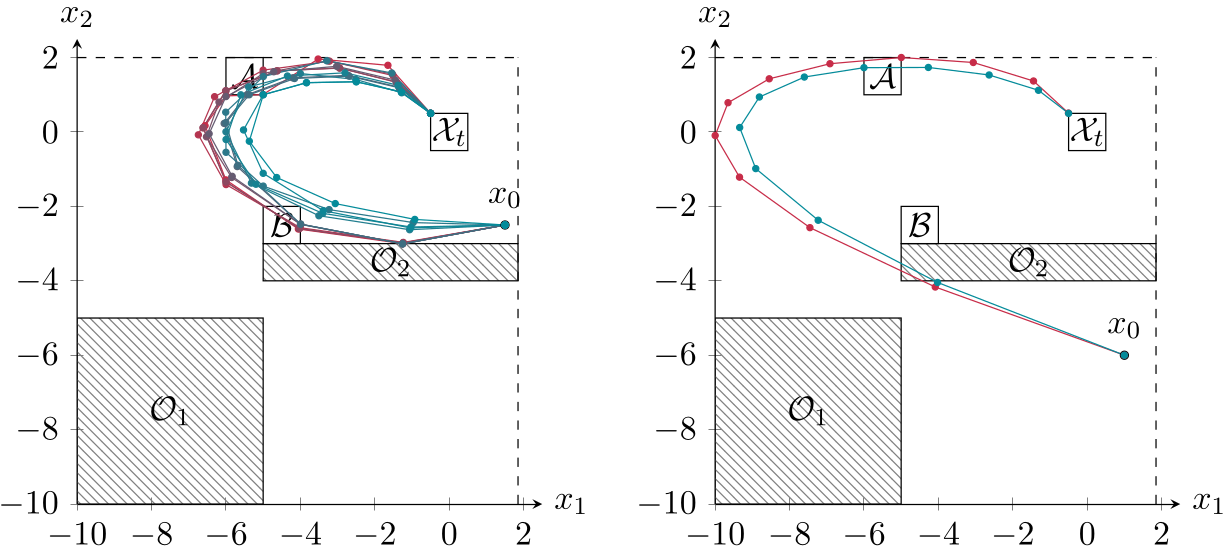
\includegraphics[width=\textwidth]{../../latex/images/abstraction-based_figs.png}
  \end{center}
  \end{block}

    \begin{minipage}{0.7\textwidth}
    The numerical results can seemlessly be reproduced using the \alert{codeocean} capsule~\cite{legat2020abstractionarXiv}.
    Algorithms implemented in the \alert{Dionysos} Julia package.%
    \end{minipage}%
    \begin{minipage}{0.3\textwidth}
    \begin{center}
      
\includegraphics[width=0.7\textwidth]{../../latex/images/Dionysos.png}
    \end{center}
    \end{minipage}

  \printbibliography
\end{column}

\end{columns} %

\end{frame}

\end{document}
